\documentclass{article}
\usepackage{gensymb, amsmath, float, graphicx}
\restylefloat{table}
\usepackage[margin=0.75in]{geometry}
\usepackage{verbatim}
\begin{document}

\title{Ocean Bowl Bootcamp 5: Ocean Layers and Sediment}
\author{Michael Shen}
\date{November 17, 2014}
\maketitle

\section{Quick Summary}

\begin{itemize}
	\item The layers of the ocean by increasing depth are: \textbf{epipelagic}, \textbf{mesopelagic}, \textbf{bathypelagic}, \textbf{abyssopelagic}, \textbf{hadopelagic} (Figure 1). The suffix \textit{-pelagic} means "open ocean" and if you know what the corresponding prefixes mean, the order becomes self-explanatory. The region of the ocean near the shore is called the \textbf{neritic zone}.
	
	\item The \textbf{photic zone} only contains the epipelagic zone. Recall that 99\% of the light is absorbed in the first 200m of the ocean and is completely absorbed by 1000m.
	
	\item \textbf{Pycnoclines} are regions where the density of water in the ocean varies greatly. An \textbf{isopycnal} is a region (typically a surface) where the density of water in the ocean is constant. There are two smaller "clines" that make up the pycnocline (Figure 2).
	\begin{itemize}
		\item \textbf{Chemoclines} are regions where concentrations of "chemicals" varies greatly. Often, this is used to mean an oxygen gradient, however a \textbf{halocline} relates to salt concentration.
		\item \textbf{Thermoclines} are regions where the temperature varies greatly.
	\end{itemize}
	
	\item There are four major types of ocean sediment: \textbf{lithogenous}, \textbf{biogenous}, \textbf{hydrogenous}, and \textbf{cosmogenous}.
	\begin{itemize}
		\item Lithogenous sediment comes in two forms: \textbf{terrigenous} (eroded rocks above the surface) and \textbf{red clay} (a mixture of terrigenous sediment and volcanic ash). 
		\begin{itemize}
			\item Terrigenous sediment is very common in rivers, while red clay is very common in the ocean. 
			\item Lithogenous sediment is dependent on the original rock, and therefore typically \textbf{silica (quartz)}.
		\end{itemize}		 
		\item Biogenous sediment comes from remains of plants and animals that do not dissolve, such as bones, teeth, shells, and coral. These are either \textbf{silica (diatoms)} or \textbf{calcium carbonate (cocolithophores)}
		\begin{itemize}
			\item In the neritic zone, it takes the form of \textbf{diatomaceous earth}, \textbf{limestone}, and \textbf{stromatolites}.
			\item In the pelagic zone, it takes the form of \textbf{siliceous and calcareous oozes}.
		\end{itemize}
		\item Hydrogenous sediment forms from the precipitation of chemicals out of the water.
		\begin{itemize}
			\item \textbf{Manganese nodules} cover approximately 70\% of the ocean floor, by far the most common hydrogenous sediment.
			\item \textbf{Metal sulfides} are created near hydrothermal vents and \textbf{salt flats} form when a region evaporates.
			\end{itemize}
		\item Cosmogenous sediment originates from outer space.
		\begin{itemize}
			\item Composed of heavy metals such as iron and nickel and can vary widely in size.
			\item Forms sediment upon impact due to the energy that can be released by impact such as \textbf{tektites} (natural glass). 
		\end{itemize}
	\end{itemize}
	
	\item I encourage everyone to look up pictures of any of the above terms that they are not familiar with. A simple Wikipedia article or Google image search will do.
	
\end{itemize}

\section{Figures}

\begin{figure}[H]
\centering
	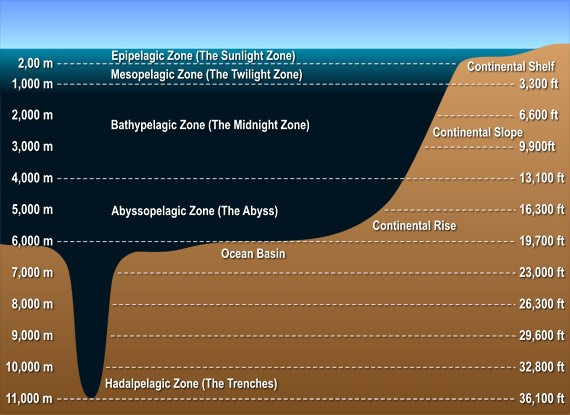
\includegraphics[scale=0.8]{./Images/BC5_OceanLayers.jpg}
	\caption{Layers of the Open Ocean}
\end{figure}
\begin{figure}[H]
\centering
	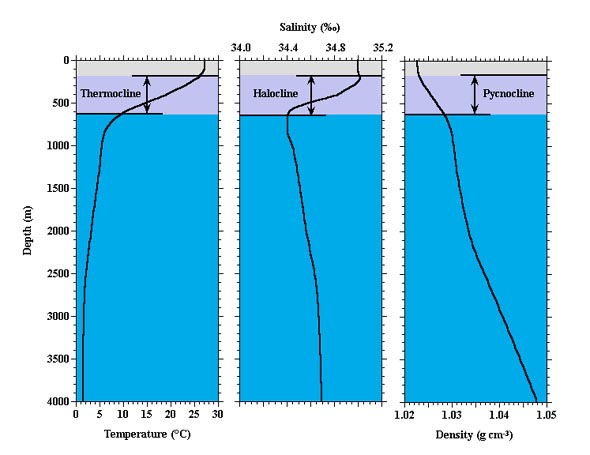
\includegraphics[scale=0.5]{./Images/BC5_Clines.jpg}
	\caption{Typical temperature, salt, and density gradients of the ocean}
\end{figure}

\end{document}